% Copyright (c) 2026 Tomás Henao

\section*{Funciones de valor real: Límites laterales} %[cite: 5]

Sea $A \subseteq \R$, $b \in \R$. %[cite: 5]

\begin{center}
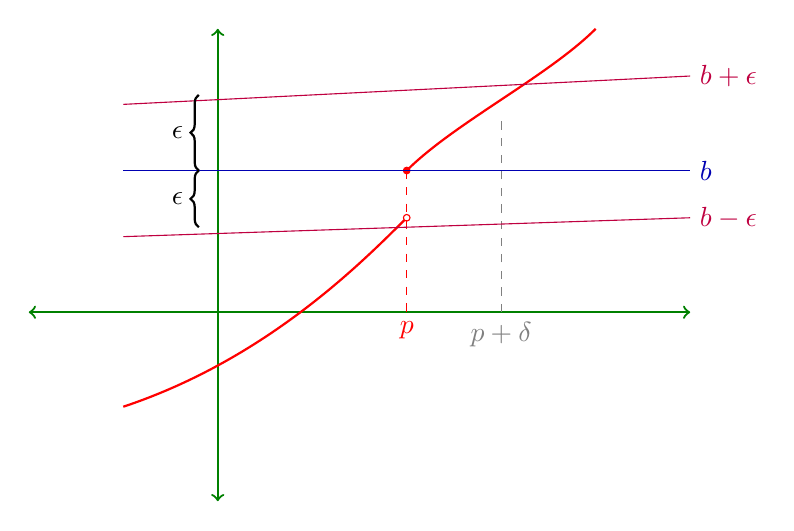
\begin{tikzpicture}[scale=1.2]
    % Ejes
    \draw[<->, thick, green!50!black] (-3,0) -- (4,0);
    \draw[<->, thick, green!50!black] (-1,-2) -- (-1,3);
    
    % Curva
    \draw[thick, red] (-2,-1) .. controls (-0.5,-0.5) and (0.5,0.5) .. (1,1);
    \draw[thick, red] (1,1.5) .. controls (1.5,2) and (2.5,2.5) .. (3,3);
    \filldraw[red] (1,1.5) circle (1pt);
    \draw[red, fill=white] (1,1) circle (1pt);
    
    % Marcas en el eje X
    \draw[dashed, red] (1,1.5) -- (1,0) node[below] {$p$};
    \draw[dashed, gray] (2,0) node[below] {$p+\delta$} -- (2,2.1);
    
    % Marcas en el eje Y (Líneas horizontales)
    \draw[blue!70!black] (-2,1.5) -- (4,1.5) node[right] {$b$};
    \draw[purple] (-2,2.2) -- (4,2.5) node[right] {$b+\epsilon$};
    \draw[purple] (-2,0.8) -- (4,1) node[right] {$b-\epsilon$};
    
    % Llaves/etiquetas de epsilon
    \draw[decoration={brace,amplitude=3pt},decorate,thick] (-1.2,1.5) -- (-1.2,2.3) node[midway,left,xshift=-2pt] {$\epsilon$};
    \draw[decoration={brace,amplitude=3pt},decorate,thick] (-1.2,0.9) -- (-1.2,1.5) node[midway,left,xshift=-2pt] {$\epsilon$};
\end{tikzpicture}
\end{center}

\begin{definicion} %[cite: 5]
Sea $f$ una función de $A$ en $\R$, $p \in A'$. %[cite: 5]
1. Decimos que el límite lateral por la derecha cuando $x$ tiende a $p$ es igual a $b$, y escribimos $f(p^+) = \lim_{x \to p^+} f(x) = b$, si y sólo si para todo $\epsilon > 0$ existe $\delta > 0$ tal que si $x \in A$ y $p < x < p + \delta$, entonces $|f(x) - b| < \epsilon$. %[cite: 5]
2. Decimos que el límite lateral por la izquierda de $f$ cuando $x$ tiende a $p$ es igual a $b$, y escribimos $f(p^-) = \lim_{x \to p^-} f(x) = b$, si y sólo si para todo $\epsilon > 0$ existe $\delta > 0$ tal que si $x \in A$ y $p - \delta < x < p$, entonces $|f(x) - b| < \epsilon$. %[cite: 5]
\end{definicion}

\begin{example} %[cite: 5]
Considere la función:
$$ f(x) = \begin{cases} 1 & \text{si } x > 0 \\ -1 & \text{si } x < 0 \end{cases} $$ %[cite: 5]
Entonces $\lim_{x \to 0^+} f(x) = 1$ y $\lim_{x \to 0^-} f(x) = -1$. %[cite: 5]
\end{example}

\begin{teorema} %[cite: 5]
Sean $A \subseteq \R$, $p \in A'$, $f$ una función de $A$ en $\R$ y $b \in \R$. %[cite: 5]
Entonces $\lim_{x \to p} f(x) = b$ si y sólo si $\lim_{x \to p^+} f(x) = b$ y $\lim_{x \to p^-} f(x) = b$. (Ejercicio). %[cite: 5]
\end{teorema}

\begin{teorema} %[cite: 5]
Si $A = [\alpha, \beta]$ con $\alpha < \beta$ y $f: A \to \R$ entonces: %[cite: 5]
a) $f$ es continua en $\beta$ si y sólo si $\lim_{x \to \beta^-} f(x) = f(\beta)$. %[cite: 5]
b) $f$ es continua en $\alpha$ si y sólo si $\lim_{x \to \alpha^+} f(x) = f(\alpha)$. (Ejercicio). %[cite: 5]
\end{teorema}

\section*{Discontinuidades de las funciones reales} %[cite: 5]

\begin{definicion} %[cite: 5]
Diremos que $p$ es un punto de discontinuidad de $f$ si $f$ no es continua en $p$. %[cite: 5]
\end{definicion}

\begin{definicion} %[cite: 5]
Supongamos que $p$ es un punto de discontinuidad de $f$. %[cite: 5]
1. Decimos que $f$ tiene una discontinuidad simple o de primera clase en $p$, si $f(p^+)$ y $f(p^-)$ existen en $\R$. %[cite: 5]
2. Decimos que $f$ tiene una discontinuidad de segunda clase en $p$ si no es simple (es decir, $f(p^+)$ o $f(p^-)$ no existen). %[cite: 5]
3. Decimos que $f$ tiene una discontinuidad evitable si presenta una discontinuidad simple en $p$ y $f(p^+) = f(p^-) \neq f(p)$. %[cite: 5]
\end{definicion}

\begin{example} %[cite: 5]
La función $f(x) = \frac{x}{|x|}$ presenta una discontinuidad simple en $x=0$, porque: %[cite: 5]
$$ |x| = \begin{cases} x & \text{si } x > 0 \\ -x & \text{si } x < 0 \end{cases} $$ %[cite: 5]
$$ \lim_{x \to 0^+} \frac{x}{|x|} = \lim_{x \to 0^+} \frac{x}{x} = \lim_{x \to 0^+} 1 = 1 $$ %[cite: 5]
$$ \lim_{x \to 0^-} \frac{x}{|x|} = \lim_{x \to 0^-} \frac{x}{-x} = \lim_{x \to 0^-} -1 = -1 $$ %[cite: 5]
Y no es evitable ya que $f(0^-) \neq f(0^+)$. %[cite: 5]
\end{example}

\begin{example} %[cite: 5]
La función $g(x) = \mathrm{sen}\left(\frac{1}{x}\right)$ presenta una discontinuidad de segunda clase en $0$. %[cite: 5]
\end{example}

\begin{teorema} %[cite: 5]
(Ejercicio) Sea $f: A \to \R$ con $A \subseteq \R$, $p \in A'$ y $b \in \R$. %[cite: 5]
a) $\lim_{x \to p^-} f(x) = b$ si y sólo si $\forall \{x_n\} \subseteq A \setminus \{p\}$ tal que $x_n \to p$ con $x_n < p$ implica que $f(x_n) \to b$. %[cite: 5]
b) $\lim_{x \to p^+} f(x) = b$ si y sólo si $\forall \{x_n\} \subseteq A \setminus \{p\}$ tal que $x_n \to p$ con $x_n > p$ implica que $f(x_n) \to b$. %[cite: 5]
\end{teorema}

\begin{remark} %[cite: 5]
Para $g(x) = \mathrm{sen}\left(\frac{1}{x}\right)$, consideremos las sucesiones $x_n = \frac{1}{2\pi n} > 0$ y $y_n = \frac{1}{\frac{\pi}{2} + 2n\pi} > 0$ con $n \in \N$. %[cite: 5]
Notar que $x_n \to 0^+$ y $y_n \to 0^+$. %[cite: 5]
1. $g(x_n) = \mathrm{sen}\left(\frac{1}{x_n}\right) = \mathrm{sen}(2\pi n) = 0$. %[cite: 5]
2. $g(y_n) = \mathrm{sen}\left(\frac{1}{y_n}\right) = \mathrm{sen}\left(\frac{\pi}{2} + 2n\pi\right) = 1$. %[cite: 5]
Entonces $\lim_{n \to \infty} g(x_n) = 0$ y $\lim_{n \to \infty} g(y_n) = 1$. %[cite: 5]
Por el teorema anterior, $\lim_{x \to 0^+} \mathrm{sen}\left(\frac{1}{x}\right)$ no existe. %[cite: 5]
\end{remark}

\begin{definicion} %[cite: 5]
Sea $f$ una función definida sobre un intervalo cerrado $[a, b]$. Si $f(c^+)$ y $f(c^-)$ existen y $c \in [a, b]$, entonces: %[cite: 5]
a) $f(c) - f(c^-)$ se llama el salto de $f$ a la izquierda de $c$. %[cite: 5]
b) $f(c^+) - f(c)$ se llama el salto de $f$ a la derecha de $c$. %[cite: 5]
c) $f(c^+) - f(c^-)$ se llama el salto de $f$ en $c$. %[cite: 5]
Si alguno de ellos es distinto de cero, entonces se dice que $f$ tiene una discontinuidad en $c$ tipo salto. %[cite: 5]
\end{definicion}

\begin{teorema}[Teorema de estricción, del emparedado o del sándwich] %[cite: 5]
Sean $f, g, h$ funciones definidas en $A \subseteq \R$, y sea $p \in A'$. %[cite: 5]
Supongamos que $f(x) \le g(x) \le h(x)$ para todo $x \in A \setminus \{p\}$ suficientemente cercano a $p$, y además $\lim_{x \to p} f(x) = L$ y $\lim_{x \to p} h(x) = L$. %[cite: 5]
Entonces $\lim_{x \to p} g(x) = L$. (El teorema es válido también para límites laterales $x \to p^+$ o $x \to p^-$). %[cite: 5]
\end{teorema}

\begin{dem} %[cite: 5]
Sea $\hat{\delta} > 0$ tal que $f(x) \le g(x) \le h(x)$ para todo $x \in A \setminus \{p\}$ con $|x - p| < \hat{\delta}$. %[cite: 5]
Veamos que $\lim_{x \to p} g(x) = L$. Sea $\epsilon > 0$, existen $\delta_1 > 0$ y $\delta_2 > 0$ tales que: %[cite: 5]
Si $x \in A \setminus \{p\}$ y $|x - p| < \delta_1$ entonces $|f(x) - L| < \epsilon \implies L - \epsilon < f(x) < L + \epsilon \quad (1)$. %[cite: 5]
Si $x \in A \setminus \{p\}$ y $|x - p| < \delta_2$ entonces $|h(x) - L| < \epsilon \implies L - \epsilon < h(x) < L + \epsilon \quad (2)$. %[cite: 5]
Tomando $\delta = \min\{\hat{\delta}, \delta_1, \delta_2\}$, tenemos que si $x \in A \setminus \{p\}$ y $|x - p| < \delta$: %[cite: 5]
$$ L - \epsilon < f(x) \le g(x) \le h(x) < L + \epsilon $$ %[cite: 5]
Luego $L - \epsilon < g(x) < L + \epsilon$, es decir, $|g(x) - L| < \epsilon$. %[cite: 5]
Por lo anterior, tenemos que $\lim_{x \to p} g(x) = L$. %[cite: 5]
\end{dem}

\begin{example} %[cite: 5]
Calcular $\lim_{x \to 0} x^2 \mathrm{sen}\left(\frac{1}{x}\right)$. %[cite: 5]
Sabemos que $-1 \le \mathrm{sen}\left(\frac{1}{x}\right) \le 1$ si $x \neq 0$. %[cite: 5]
Multiplicando por $x^2 > 0$: $-x^2 \le x^2 \mathrm{sen}\left(\frac{1}{x}\right) \le x^2$ si $x \neq 0$. %[cite: 5]
Como $\lim_{x \to 0} -x^2 = 0$ y $\lim_{x \to 0} x^2 = 0$, %[cite: 5]
por el teorema de estricción tenemos $\lim_{x \to 0} x^2 \mathrm{sen}\left(\frac{1}{x}\right) = 0$. %[cite: 5]
\end{example}

\begin{remark} %[cite: 5]
Ejercicio: $\lim_{x \to 0^+} x \mathrm{sen}\left(\frac{1}{x}\right)$. %[cite: 5]
Usando la función $-1 \le \mathrm{sen}\left(\frac{1}{x}\right) \le 1$ para $x \neq 0$. %[cite: 5]
Con $x > 0$, tenemos: $-x \le x \mathrm{sen}\left(\frac{1}{x}\right) \le x$. %[cite: 5]
Aplicando el límite, el resultado también es $0$. %[cite: 5]
\end{remark}

\section*{Límites infinitos y en el infinito} %[cite: 5]

\begin{definicion}[Límites infinitos] %[cite: 5]
Sea $f$ una función de valor real definida en $A \subseteq \R$ y $p \in A'$. %[cite: 5]
1. Decimos $\lim_{x \to p} f(x) = \infty$ si y sólo si para todo número real $M > 0$ existe $\delta > 0$ tal que si $x \in A \setminus \{p\}$ y $|x - p| < \delta$ implica $f(x) > M$. %[cite: 5]
2. Decimos $\lim_{x \to p} f(x) = -\infty$ si y sólo si para todo número real $M > 0$ existe $\delta > 0$ tal que si $x \in A \setminus \{p\}$ y $|x - p| < \delta$ implica $f(x) < -M$. %[cite: 5]
\end{definicion}

\begin{example} %[cite: 5]
$\lim_{x \to 0} \frac{1}{x^2} = \infty$. %[cite: 5]
En efecto, sea $M > 0$, existe $\delta = \frac{1}{\sqrt{M}}$ tal que si $|x| < \frac{1}{\sqrt{M}}$ entonces $x^2 < \frac{1}{M}$. %[cite: 5]
Sea $x \neq 0$, si $0 < |x| < \delta$ entonces $x^2 < \frac{1}{M}$, lo que implica $\frac{1}{x^2} > M$. %[cite: 5]
Por lo anterior $\lim_{x \to 0} \frac{1}{x^2} = \infty$. %[cite: 5]
\end{example}

\begin{definicion}[Límites en el infinito] %[cite: 5]
Sea $f: \R \to \R$ una función, decimos: %[cite: 5]
1. $\lim_{x \to \infty} f(x) = L$ si y sólo si para todo $\epsilon > 0$ existe $M > 0$ tal que si $x > M$ entonces $|f(x) - L| < \epsilon$. %[cite: 5]
2. $\lim_{x \to -\infty} f(x) = L$ si y sólo si para todo $\epsilon > 0$ existe $M > 0$ tal que si $x < -M$ entonces $|f(x) - L| < \epsilon$. %[cite: 5]
\end{definicion}

\begin{teorema} %[cite: 5]
$\lim_{x \to \infty} f(x) = L$ si y sólo si para toda sucesión $\{x_n\} \subseteq \R$ tal que $x_n \to \infty$ cuando $n \to \infty$ implica que $f(x_n) \to L$. %[cite: 5]
(Recordar: $\lim_{n \to \infty} x_n = \infty$ si y sólo si $(\forall M > 0)(\exists N \in \N)(\forall n \ge N)$ entonces $x_n > M$). %[cite: 5]
\end{teorema}

\begin{dem} %[cite: 5]
($\implies$) Supongamos que $\lim_{x \to \infty} f(x) = L$. %[cite: 5]
Sea $\{x_n\} \subseteq \R$ tal que $x_n \to \infty$ cuando $n \to \infty$. Veamos que $\lim_{n \to \infty} f(x_n) = L$. %[cite: 5]
Sea $\epsilon > 0$, existe $M > 0$ tal que si $x > M$ entonces $|f(x) - L| < \epsilon$. %[cite: 5]
Como $x_n \to \infty$, usando la definición con $M > 0$, existe $N \in \N$ tal que para todo $n \ge N$, $x_n > M$. %[cite: 5]
Por lo anterior tenemos que si $n \ge N$, $x_n > M$, y por tanto $|f(x_n) - L| < \epsilon$. Es decir $f(x_n) \to L$. %[cite: 5]

($\impliedby$) Supongamos por contradicción que $\lim_{x \to \infty} f(x) \neq L$. %[cite: 5]
Es decir, existe $\epsilon_0 > 0$ tal que para todo $M > 0$ existe $x \in \R$ con $x > M$ y $|f(x) - L| \ge \epsilon_0$. %[cite: 5]
Para cada $n \in \N$, tomando $M = n$, existe $x_n \in \R$ tal que $x_n > n$ y $|f(x_n) - L| \ge \epsilon_0$. %[cite: 5]
Notar que $x_n \to \infty$ cuando $n \to \infty$ (ejercicio). %[cite: 5]
Por hipótesis $f(x_n) \to L$. ¡Contradicción! %[cite: 5]
Pues con $\epsilon = \epsilon_0$ existiría un $N \in \N$ tal que $|f(x_n) - L| < \epsilon_0$ para $n \ge N$. %[cite: 5]
\end{dem}

\section*{Funciones monótonas} %[cite: 5]

\begin{definicion} %[cite: 5]
Sea $f$ una función real definida en un subconjunto $A$ de $\R$. Entonces: %[cite: 5]
1. $f$ es creciente (o no decreciente) en $A$ si para todo $x, y \in A$ tales que $x < y$ implica $f(x) \le f(y)$. %[cite: 5]
2. Decimos que $f$ es estrictamente creciente en $A$ si para todo $x, y \in A$ tales que $x < y$ entonces $f(x) < f(y)$. %[cite: 5]
3. Si la última desigualdad es $f(x) \ge f(y)$ (o $f(x) > f(y)$), decimos que $f$ es decreciente (o estrictamente decreciente) en $A$. %[cite: 5]
4. Una función es monótona en $A$ si es creciente o decreciente en $A$. %[cite: 5]
\end{definicion}

\begin{teorema} %[cite: 5]
Sea $f: (a,b) \to \R$ una función monótona en $(a,b)$. Entonces para $c \in (a,b)$, $f(c^+)$ y $f(c^-)$ existen. %[cite: 5]
Además: %[cite: 5]
1. Si $f$ es creciente en $(a,b)$ entonces $f(c^-) = \sup\{f(x) \mid a < x < c\} \le f(c) \le \inf\{f(x) \mid c < x < b\} = f(c^+)$. %[cite: 5]
2. Si $f$ es decreciente en $(a,b)$ entonces $f(c^-) = \inf\{f(x) \mid a < x < c\} \ge f(c) \ge \sup\{f(x) \mid c < x < b\} = f(c^+)$. %[cite: 5]
\end{teorema}

\begin{dem} %[cite: 5]
\textbf{Prueba de (1):} Si $f$ es creciente en $(a,b)$. %[cite: 5]
Sea $A = \{f(x) \mid a < x < c\}$. Notemos que $A$ está acotado superiormente por $f(c)$, pues $f$ es una función creciente. %[cite: 5]
Sea $\alpha = \sup A$. Queremos probar que $\lim_{x \to c^-} f(x) = \alpha$, es decir $\alpha \le f(c)$. %[cite: 5]
Sea $\epsilon > 0$. Queremos hallar $\delta > 0$ tal que si $x \in (a,b)$ y $c - \delta < x < c$ entonces $|f(x) - \alpha| < \epsilon$ (es decir, $\alpha - \epsilon < f(x) < \alpha + \epsilon$). %[cite: 5]
Por la caracterización de supremo, existe $x_1 < c$ tal que $\alpha - \epsilon < f(x_1) \le \alpha$. %[cite: 5]
Tomando $\delta = c - x_1 > 0$, tenemos que si $x \in (a,b)$ y $x \in (c-\delta, c) = (x_1, c)$, como $f$ es creciente, $\alpha - \epsilon < f(x_1) \le f(x) \le \alpha < \alpha + \epsilon$. %[cite: 5]
Entonces $\alpha - \epsilon < f(x) < \alpha + \epsilon$, por tanto $|f(x) - \alpha| < \epsilon$. %[cite: 5]

Sea $B = \{f(x) \mid c < x < b\}$. Claramente $f(c)$ es una cota inferior para el conjunto $B$. %[cite: 5]
Sea $\beta = \inf B$, y sabemos $f(c) \le \beta$. Sea $\epsilon > 0$. %[cite: 5]
Por la caracterización de ínfimo, existe $c < x_2 < b$ tal que $\beta \le f(x_2) < \beta + \epsilon$. %[cite: 5]
Tomando $\delta = x_2 - c$, tenemos que si $x \in (a,b)$ y $x \in (c, c+\delta) = (c, x_2)$, %[cite: 5]
$\beta - \epsilon < \beta \le f(x) \le f(x_2) < \beta + \epsilon$. %[cite: 5]
Por lo anterior $f(c^+) = \beta = \inf B$. %[cite: 5]

\textbf{Prueba de (2):} (Ejercicio). Supongamos que $f$ es decreciente en $(a,b)$. %[cite: 5]
Recordar: Si $D \subseteq \R$ tiene acotado, $\sup(-D) = -\inf D$ y $\inf(-D) = -\sup D$, donde $-D = \{-x \mid x \in D\}$. %[cite: 5]
Si $f$ es decreciente, entonces $-f$ es creciente en $(a,b)$. Por (1) tenemos: %[cite: 5]
$(-f)(c^-) = \sup\{-f(x) \mid a < x < c\} \le -f(c) \le \inf\{-f(x) \mid c < x < b\} = (-f)(c^+)$. %[cite: 5]
Es decir: $-\inf\{f(x) \mid a < x < c\} \le -f(c) \le -\sup\{f(x) \mid c < x < b\}$. %[cite: 5]
Multiplicando por $-1$: $\inf\{f(x) \mid a < x < c\} \ge f(c) \ge \sup\{f(x) \mid c < x < b\}$. %[cite: 5]
\end{dem}

\begin{corolario} %[cite: 5]
(Ejercicio). Sea $f: (a,b) \to \R$ una función monótona, entonces $f$ no tiene discontinuidades de segunda clase. %[cite: 5]
\end{corolario}

\begin{teorema} %[cite: 5]
Sea $f$ una función monótona en $(a,b)$. El conjunto de puntos en $(a,b)$ en los cuales $f$ es discontinua es a lo sumo numerable. %[cite: 5]
\end{teorema}

\begin{dem} %[cite: 5]
Supongamos sin pérdida de generalidad que $f$ es creciente. %[cite: 5]
Por el teorema anterior tenemos que para todo $c \in (a,b)$, $f(c^-) \le f(c) \le f(c^+)$. %[cite: 5]
Definimos $D = \{x \in (a,b) \mid f \text{ es discontinua en } x\}$. %[cite: 5]
Por el corolario anterior, las discontinuidades son de primera clase. %[cite: 5]

\textbf{Afirmación 1:} Si $x \in D$ entonces $f(x^-) < f(x^+)$. %[cite: 5]
Supongamos por contradicción que $f(x^-) \ge f(x^+)$. %[cite: 5]
Como $f$ es creciente, por teorema anterior $f(x^-) \le f(x^+)$. %[cite: 5]
Luego $f(x^+) = f(x) = f(x^-)$. ¡Contradicción! Porque $f$ es discontinua en $x$. %[cite: 5]

\textbf{Afirmación 2:} Si $x, y \in D$ con $x < y$ entonces $f(x^+) \le f(y^-)$. %[cite: 5]
Supongamos por contradicción $f(x^+) > f(y^-)$. %[cite: 5]
$f(y^-) = \sup\{f(t) \mid a < t < y\} < f(x^+) = \inf\{f(t) \mid x < t < b\}$. %[cite: 5]
En particular para un $\hat{t} \in (x,y)$ (porque $x < y$), $f(x^+) > f(\hat{t})$. %[cite: 5]
Pero $f(x^+) \le f(t)$ para todo $t \in (x,b)$, ¡contradicción! %[cite: 5]
Luego $f(x^+) \le f(y^-)$. %[cite: 5]

Para $x \in D$, de la afirmación 1 tenemos que el intervalo $(f(x^-), f(x^+))$ es no vacío, entonces existe $q_x \in \Q$ tal que $q_x \in (f(x^-), f(x^+))$ (porque $\Q$ es denso en $\R$). %[cite: 5]

\textbf{Afirmación 3:} Si $x,y \in D$ con $x < y$ entonces $(f(x^-), f(x^+)) \cap (f(y^-), f(y^+)) = \emptyset$. %[cite: 5]
Es claro, de la afirmación 2 ($f(x^+) \le f(y^-)$). %[cite: 5]

\textbf{Afirmación 4:} Si $x, y \in D$ y $x \neq y$ entonces $q_x \neq q_y$. %[cite: 5]
Es claro de la afirmación 3. %[cite: 5]

Por lo anterior, la función $g: D \to \Q$ definida por $x \mapsto g(x) = q_x$ es inyectiva por la afirmación 4. %[cite: 5]
Entonces $D$ es a lo sumo numerable. %[cite: 5]
\end{dem}

\begin{teorema} %[cite: 5]
Sea $f$ estrictamente creciente en un conjunto $A \subseteq \R$, entonces $f^{-1}$ existe y es estrictamente creciente en $f(A)$. (Ejercicio). %[cite: 5]
\end{teorema}

\begin{teorema} %[cite: 5]
Sea $f$ estrictamente creciente y continua en un intervalo compacto $[a,b]$. %[cite: 5]
Entonces $f^{-1}$ es estrictamente creciente y continua en el intervalo $[f(a), f(b)]$. (Ejercicio). %[cite: 5]
\end{teorema}